%
% $RCSfile: presentation_client.tex,v $
%
% Copyright (C) 2002-2008. Christian Heller.
%
% Permission is granted to copy, distribute and/or modify this document
% under the terms of the GNU Free Documentation License, Version 1.1 or
% any later version published by the Free Software Foundation; with no
% Invariant Sections, with no Front-Cover Texts and with no Back-Cover
% Texts. A copy of the license is included in the section entitled
% "GNU Free Documentation License".
%
% http://www.cybop.net
% - Cybernetics Oriented Programming -
%
% http://www.resmedicinae.org
% - Information in Medicine -
%
% Version: $Revision: 1.1 $ $Date: 2008-08-19 20:41:08 $ $Author: christian $
% Authors: Christian Heller <christian.heller@tuxtax.de>
%

\section{Presentation Client}
\label{presentation_client_heading}
\index{Presentation Client}
\index{Client}
\index{3 Tiers}
\index{Remote Method Invocation}
\index{RMI}
\index{Remote Procedure Call}
\index{RPC}
\index{Thin Client}
\index{Fat Client}
\index{Rich Client}

A system is called \emph{Client} when it uses services of a server. Most modern
applications incorporate abilities to communicate with server systems which may
run on the same computer as the client or on a remote machine that has to be
accessed over network.

\begin{figure}[ht]
    \begin{center}
        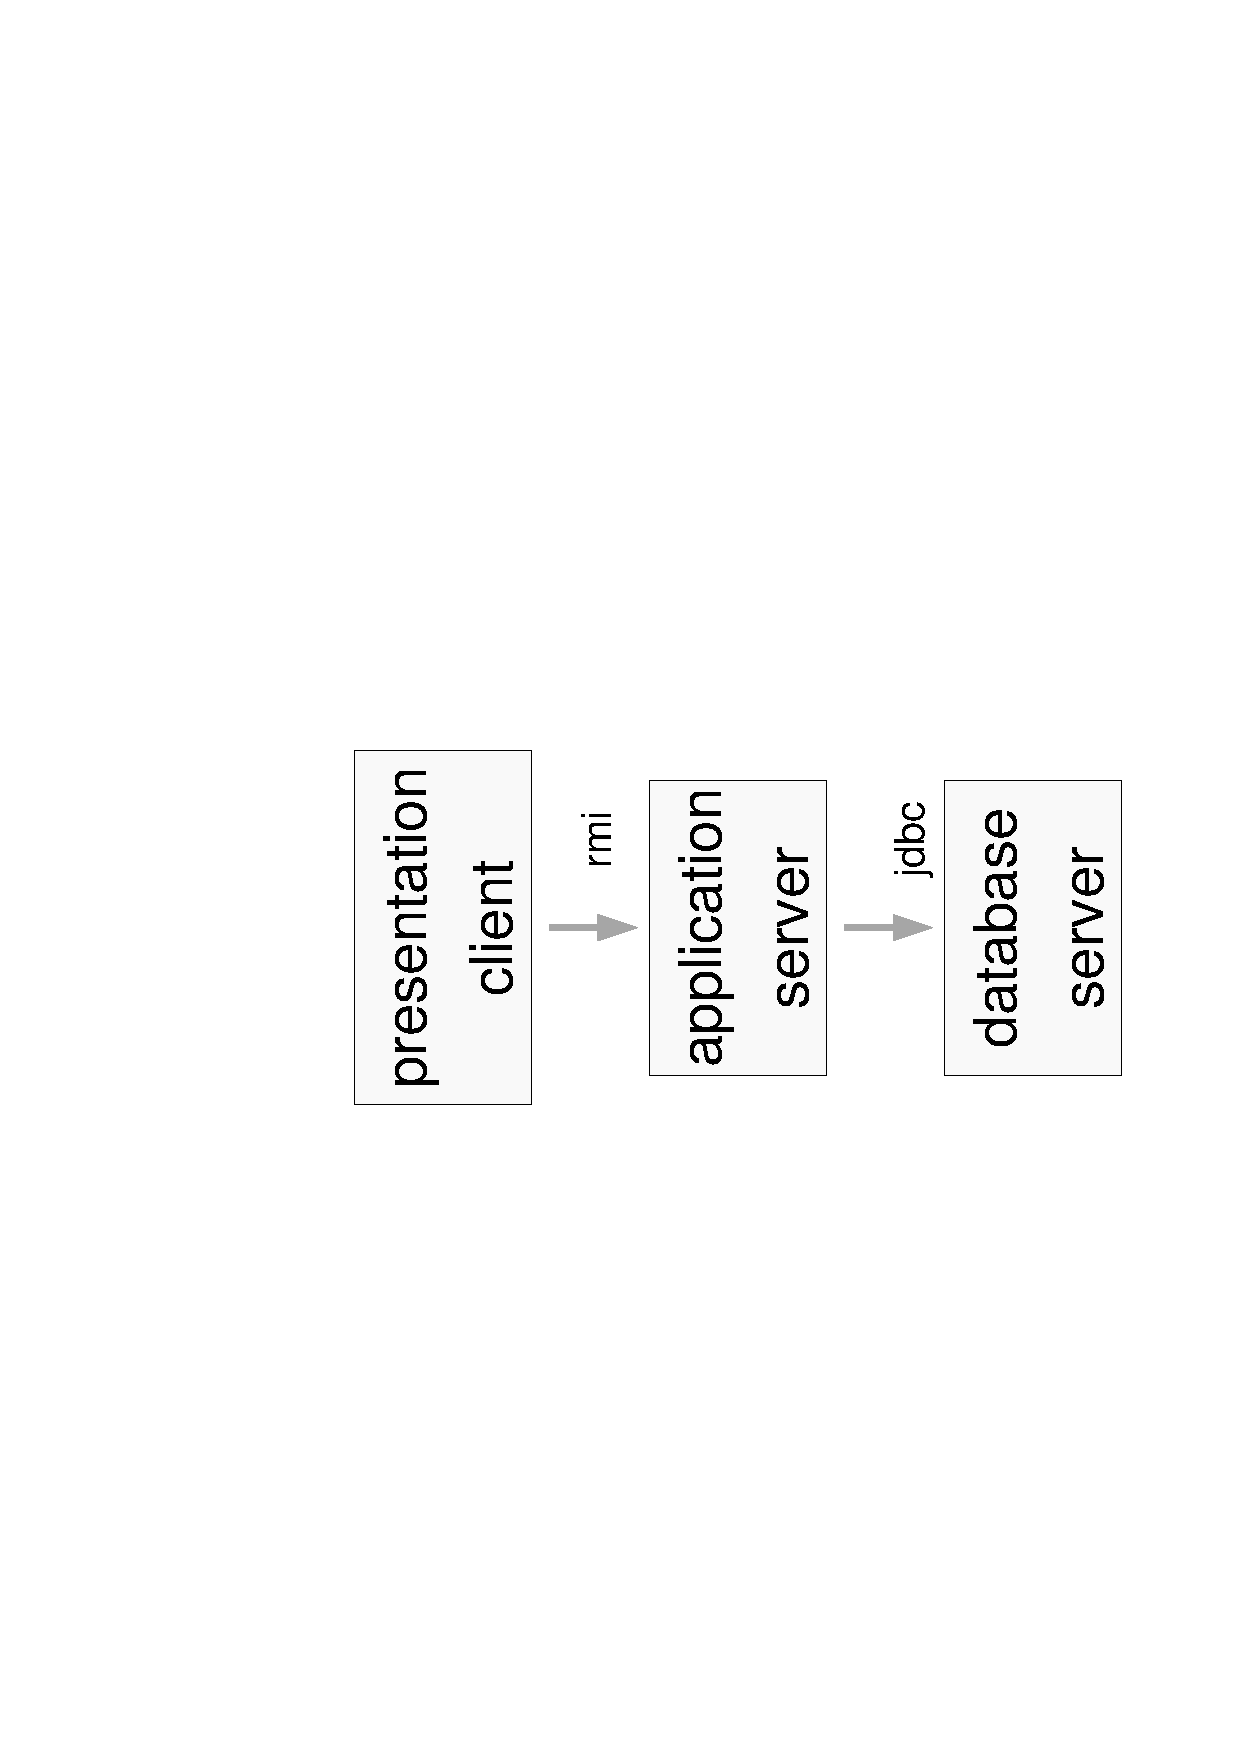
\includegraphics[scale=0.3,angle=-90]{graphic/client.pdf}
        \caption{Presentation Client (3 Tiers)}
        \label{client_figure}
    \end{center}
\end{figure}

But also clients can offer services as well as servers can use external services
and such become clients themselves. The application server in figure
\ref{database_figure} becomes a client when accessing the database system.
As can be seen -- \emph{Client} and \emph{Server} are quite arbitrary terms to
characterise systems.

Figure \ref{client_figure} illustrates the communication between a presentation
client and application server over network. Again, various mechanisms such as
\emph{Remote Method Invocation} (RMI), outside the Java world rather called
\emph{Remote Procedure Call} (RPC), exist to ease the way two remote systems
talk with one another.

Frequently, people distinguish between \emph{Thin Client} and \emph{Fat Client}
(the latter also called \emph{Rich Client}) \cite[p. 176]{zimmermann}. While a
thin client's task is nothing else than to display information coming from some
server, a fat client also takes over part of the business data processing which
is otherwise done by the server only.
